\documentclass[11pt]{article}

% --- Packages -------------------------------------------------------------
\usepackage[utf8]{inputenc}
\usepackage[T1]{fontenc}
\usepackage{lmodern}
\usepackage{amsmath, amssymb, mathtools}
\usepackage{bm}
\usepackage{graphicx}
\usepackage{xcolor}
\usepackage{hyperref}
\usepackage[capitalize,noabbrev]{cleveref}
\usepackage{geometry}
\usepackage{caption}
\usepackage{subcaption}
\usepackage[numbers]{natbib}
\geometry{a4paper, margin=2.4cm}

% --- Notation lifted from companion papers --------------------------------
\newcommand{\bxi}{\boldsymbol{\xi}}
\newcommand{\bx}{\bm{x}}
\newcommand{\avg}[1]{\langle #1 \rangle}
\newcommand{\e}{{\mathrm{e}}}
\newcommand{\dd}{{\mathrm{d}}}
\newcommand{\Bnet}{\beta_{\mathrm{net}}}
\newcommand{\phieq}{\phi_{\mathrm{eq}}}
\newcommand{\fret}{f_{\mathrm{ret}}}
\newcommand{\acGauss}{\alpha_c^{\mathrm{G}}}
\newcommand{\acBd}{\alpha_c^{\mathrm{bd}}}
\newcommand{\acSd}{\alpha_c^{\mathrm{sd}}}
\newcommand{\acSp}{\alpha_c^{\mathrm{sp}}}

\title{\bfseries Saddle-Dominated Capacity of LSE Dense Associative Memory}
\author{}
\date{}

\begin{document}
\maketitle

% =========================================================================
\begin{abstract}
\noindent
The classical capacity argument of Ramsauer et al.\ for the log-sum-exp (LSE)
energy on the $N$-sphere places the storage threshold at $\alpha_c = 0.5$ in
the $N\!\to\!\infty$ limit. That argument is static, formulated at $T=0$, and
carries no notion of basin stability against thermal noise. Recasting the
problem as a thermodynamic competition between energy and geometric entropy
recovers the same $0.5$ at $T\!\to\!0$ under a Gaussian approximation for the
inter-pattern overlap distribution. A companion analysis for the
compactly-supported log-sum-ReLU (LSR) kernel showed that the Gaussian
overstates the tails of that distribution: replacing it by the exact
spherical density $f(\varphi)\propto(1-\varphi^2)^{(N-3)/2}$ shifts the LSR
threshold to $-\tfrac12\ln(1-\varphi_c^2)\approx0.347$. The same lighter-tail
correction applied to LSE does \emph{not} reduce to a single boundary
formula: the exponential kernel of LSE creates an interior saddle in the
spurious-sum integrand at the \emph{golden ratio}
$\varphi^{*} = (\sqrt{5}-1)/2 \approx 0.618$, yielding
$\acSd(T) = \Bnet - g_{\max} - \fret(T) \approx 0.6226 - \fret(T)$ with
$\Bnet = 1$. The corrected $T\!\to\!0$ capacity is the golden constant
$\approx 0.6226$, neither the Ramsauer value of $0.5$ nor the divergent
boundary form one obtains by naive transplant from LSR. Honest $N=25$ Monte
Carlo over $\alpha\in[0.20,0.70]$, cross-checked against a saddle-band
retaining truncation in the high-$\alpha$ memory-bound regime, supports the
saddle prediction for $\alpha\gtrsim0.45$.
\end{abstract}

% =========================================================================
\section{Introduction}
\label{sec:intro}

The modern Hopfield network of Krotov and Hopfield~\citep{krotov2016dense}
replaces the pairwise interaction of the classical model by a continuous
energy function with exponential storage capacity. The dot-product form
\begin{equation}
H_{\mathrm{LSE}}(\bx) \;=\; -\frac{1}{\Bnet}\,\ln\!
\Bigl(\sum_{\mu=1}^{M} \exp(\Bnet\,\bx\cdot\bxi^\mu)\Bigr),
\label{eq:lse-energy}
\end{equation}
with $M$ stored patterns $\bxi^\mu$ on the $N$-sphere of radius $\sqrt{N}$,
was popularised by Ramsauer et al.~\citep{ramsauer2021hopfield} together
with the capacity statement that retrieval is possible up to
$\alpha = \ln(M)/N \le 1/2$. Their argument rests on a static condition
(the queried pattern's overlap with the state exceeds that of every other
pattern, with high probability) under the assumption that inter-pattern
alignments $\varphi_{1\mu} = \bxi^1\!\cdot\bxi^\mu / N$ are well approximated
by a Gaussian of variance $1/N$. The analysis is performed at $T=0$ and does
not address whether the state $\bx\!\approx\bxi^1$ remains a stable basin of
attraction under thermal fluctuations.

A finite-temperature treatment was given by the
companion paper~\citep{icml2026theory}, which casts retrieval as a
competition between the kernel-dependent internal energy and the geometric
entropy $s(\varphi) = \tfrac12 \ln(1-\varphi^2)$ of the $N$-sphere. Within
the same Gaussian assumption, this thermodynamic formulation recovers
$\alpha_c(0) = 1/2$ for LSE and predicts a smooth boundary
$\acGauss(T) = \tfrac12[1-\fret(T)]^2$ separating the retrieval phase from
the spin-glass phase, where
\begin{align}
\phieq(T)   &= \tfrac12\bigl(-T + \sqrt{T^2+4}\bigr),
\label{eq:phieq}\\
\fret(T)    &= 1 - \phieq(T) - \tfrac{T}{2}\,\ln\!\bigl(1-\phieq(T)^2\bigr).
\label{eq:fret}
\end{align}

A follow-up analysis~\citep{petrova2026metastable} revisited the Gaussian
assumption for the compactly-supported LSR kernel
$\max\bigl(0,\;1-b+b\,\varphi\bigr)$. The true overlap density on the
$N$-sphere,
\begin{equation}
f(\varphi) \;=\; \frac{(1-\varphi^2)^{(N-3)/2}}
                       {B\!\bigl((N-1)/2,\,1/2\bigr)},
\qquad \varphi\in[-1,1],
\label{eq:exact-density}
\end{equation}
shares mean and variance with the moment-matched Gaussian but has lighter
tails: it vanishes at $|\varphi|=1$, whereas the Gaussian assigns
nonzero weight there. For LSR the hard cutoff $\varphi_c = (b-1)/b$
combines with the lighter tail to push the threshold up from
$\varphi_c^2/2$ (Gaussian) to $-\tfrac12 \ln(1-\varphi_c^2)$. With
$b = 2+\sqrt{2}$ this is a shift from $0.25$ to $\approx 0.347$.

The question pursued in this paper is the LSE analogue. Naively transplanting
the LSR formula, by retaining only the lighter-tail spherical density and
identifying the support boundary $\varphi_{\max}$ from the typical maximum
overlap of $M$ patterns, gives
$\acBd(T) = -\tfrac12\ln\bigl[1-(1-\fret(T))^2\bigr]$, which diverges as
$T\!\to\!0$ and over-predicts capacity catastrophically against Monte Carlo.
We argue and demonstrate that this transplant is wrong for a structural
reason: the exponential kernel of LSE multiplies the lighter-tail density by
$\e^{\Bnet N \varphi}$, and the resulting exponent
$g(\varphi) = \tfrac12 \ln(1-\varphi^2) + \Bnet\,\varphi$ has a stationary
point strictly inside the support of $\varphi$. The spurious sum is dominated
not by the support boundary but by an interior saddle, which for $\Bnet=1$
sits exactly at the \emph{golden ratio} $\varphi^* = (\sqrt{5}-1)/2$. The
corrected capacity is
$\acSd(T) = \Bnet - g_{\max} - \fret(T)$ with $g_{\max} \approx 0.3774$, so
$\acSd(0) \approx 0.6226$. Ramsauer's $0.5$ must be reconsidered: in the
$T\!\to\!0$ limit of the thermodynamic boundary, the lighter-tail correction
raises the capacity to a golden constant intermediate between the Gaussian
estimate and the divergent boundary form. Honest Monte Carlo at $N=25$ over
$\alpha\in[0.20,0.70]$, supplemented at high $\alpha$ by a quenched
saddle-band-retaining truncation, supports the saddle prediction in the
regime where finite-$N$ kinetic effects are mild.

% =========================================================================
\section{Three predictions for $\alpha_c(T)$}
\label{sec:formulas}

The starting point is the spurious-sum noise floor for a chain held at the
retrieval state $\bx\!\approx\!\bxi^1$. The retrieval term contributes
$\exp(\Bnet N)$ to the partition function summand
\eqref{eq:lse-energy}; the remaining $M-1$ patterns contribute
\begin{equation}
S_{\mathrm{spurious}} \;=\; \sum_{\mu\neq 1}
   \exp\!\bigl(\Bnet\,N\,\varphi_{1\mu}\bigr)
   \;\approx\; M \int_{-1}^{1} f(\varphi)\,
        \exp\!\bigl(\Bnet\,N\,\varphi\bigr)\,\dd\varphi.
\label{eq:spurious-sum}
\end{equation}
At $T=0$ the retrieval-to-spin-glass crossover occurs when
$S_{\mathrm{spurious}}$ overwhelms the retrieval contribution
$\exp(\Bnet N)$; at finite $T$ the same condition becomes the equality of
the retrieval free energy $\fret(T)$ \eqref{eq:fret} with the noise floor
$u_{\mathrm{noise}}(\alpha)$. Three predictions for the boundary
$\acGauss, \acBd, \acSd$ follow, distinguished by which density
$f(\varphi)$ is used in \eqref{eq:spurious-sum} and where the integrand
attains its maximum on the relevant support.

\paragraph{Gaussian regime (Ramsauer / ICML).}
Replacing $f(\varphi)$ by the moment-matched Gaussian
$\sqrt{N/2\pi}\,\exp(-N\varphi^2/2)$, the integrand exponent
$-\varphi^2/2 + \Bnet\,\varphi$ is monotone increasing on $[-1,1]$ and
dominated by the right boundary at $\varphi = 1$ with value
$\Bnet - 1/2$. Substituting into the crossover condition yields
$u_{\mathrm{noise}}^{\mathrm{G}}(\alpha) = 1 - \sqrt{2\alpha}$ and
\begin{equation}
\acGauss(T) \;=\; \tfrac12\bigl[1 - \fret(T)\bigr]^2,
\qquad \acGauss(0) = 1/2,
\label{eq:acgauss}
\end{equation}
recovering the Ramsauer value as the zero-temperature limit. This boundary
is the LSE prediction of~\citep{icml2026theory}.

\paragraph{Exact-density boundary regime.}
Retaining the exact spherical density \eqref{eq:exact-density} but
restricting attention to the support edge
$\varphi_{\max}(\alpha) = \sqrt{1 - \e^{-2\alpha}}$, i.e.\ the typical
maximum overlap among $M = \e^{\alpha N}$ random unit vectors, gives
$u_{\mathrm{noise}}^{\mathrm{bd}}(\alpha) = 1 - \varphi_{\max}(\alpha)$ and
\begin{equation}
\acBd(T) \;=\; -\tfrac12\,\ln\!\bigl[\,1 - (1-\fret(T))^2\,\bigr],
\qquad \acBd(0) \to +\infty.
\label{eq:acbd}
\end{equation}
This is the formula one obtains by transplanting the LSR derivation
of~\citep{petrova2026metastable} to LSE. As shown in
\Cref{sec:formulas:saddle}, it is correct only at $\alpha$ below the
regime split defined in \Cref{sec:formulas:split}, which lies far to the
left of the entire $\alpha$ range studied here.

\paragraph{Exact-density saddle regime (this work).}
\label{sec:formulas:saddle}
On the unbounded support $[-1,1]$ the integrand of \eqref{eq:spurious-sum}
with $f$ from \eqref{eq:exact-density} has exponent
$g(\varphi) = \tfrac12 \ln(1-\varphi^2) + \Bnet\,\varphi$. The stationarity
condition $g'(\varphi)=0$ reads $\Bnet(1-\varphi^2) = \varphi$, which for
$\Bnet = 1$ becomes
\begin{equation}
\varphi^{*\,2} + \varphi^{*} - 1 \;=\; 0
\;\;\Longrightarrow\;\;
\varphi^{*} \;=\; \frac{\sqrt{5}-1}{2} \;\approx\; 0.618 \;\; \text{(golden ratio).}
\label{eq:phistar}
\end{equation}
The identity $1 - \varphi^{*\,2} = \varphi^{*}$ gives the saddle value
\begin{equation}
g_{\max} \;=\; \tfrac12 \ln \varphi^{*} + \varphi^{*}
        \;\approx\; 0.3774.
\label{eq:gmax}
\end{equation}
Substituting into the spurious-to-retrieval crossover
$\alpha + g_{\max} = \Bnet$ at $T=0$ and equating with $\fret(T)$ at
finite $T$ yields the corrected boundary
\begin{equation}
\boxed{\;
\acSd(T) \;=\; \Bnet - g_{\max} - \fret(T) \;\approx\; 0.6226 - \fret(T),
\qquad \acSd(0) \approx 0.6226.
\;}
\label{eq:acsd}
\end{equation}
The zero-temperature limit is the golden constant
$\Bnet - g_{\max} = 1 - \tfrac12 \ln \varphi^{*} - \varphi^{*}
\approx 0.6226$, neither $1/2$ (Gaussian) nor $\infty$ (boundary
transplant).

\paragraph{Regime split.}
\label{sec:formulas:split}
The saddle \eqref{eq:phistar} lies inside the natural support
$[0,\varphi_{\max}(\alpha)]$ precisely when
$\varphi^{*} \le \varphi_{\max}(\alpha)$, i.e.\ when
$\alpha \ge -\tfrac12 \ln(1-\varphi^{*\,2}) = -\tfrac12 \ln \varphi^{*}
\approx 0.241$. For $\alpha < 0.241$ the integrand is monotone on the
available support and the boundary form $\acBd$ applies; for
$\alpha \ge 0.241$ the saddle form $\acSd$ applies. The Monte Carlo
window of this paper, $\alpha \in [0.20, 0.70]$, sits almost entirely in
the saddle regime; the orange-dashed and red-solid curves
\eqref{eq:acbd},\eqref{eq:acsd} meet at $\alpha \approx 0.241$ on the
plotted axes (\Cref{fig:heatmap}).

% =========================================================================
\section{Monte Carlo}
\label{sec:mc}

We test the three predictions of \Cref{sec:formulas} against direct
simulation. All chains are run on the $N$-sphere with $\Bnet = 1$,
Metropolis updates, step size $\sigma(T) = 2.4\,T/\sqrt{N}$, and chain
length $N_{\mathrm{EQ}} = 2^{15} = 32{,}768$ unmeasured equilibration steps
followed by $N_{\mathrm{SAMP}} = 2^{13} = 8{,}192$ sampling steps. Two
replicas per disorder sample are initialised at the retrieval pattern
$\bxi^1$; we report the per-cell residual
$\avg{\phi} - \phieq(T)$, averaged over disorder seeds. The $\alpha$ grid
is $[0.20,\,0.70]$ in steps of $0.01$; the $T$ grid is $40$ increasing
points $\mathrm{range}(0.025,\,0.500,\,40)$, excluding $T=0$.

\subsection{Honest MC}
\label{sec:mc:honest}

In the honest scheme all $M = \lceil \e^{\alpha N}\rceil$ patterns are
generated explicitly as $\bxi^\mu \sim \mathrm{Unif}\bigl(\sqrt{N}\,
S^{N-1}\bigr)$. The target spin count is $N = 25$, chosen so that
$M$ at $\alpha = 0.70$ is on the order of $4\times10^7$, near the
edge of single-GPU pattern-storage feasibility. The script applies a
memory-aware fallback: at each $\alpha$ it caps the per-$\alpha$ disorder
multiplicity to fit a configurable budget ($40~\mathrm{GB}$ here), and
drops $N$ in unit steps only if a single disorder sample still does not
fit. The per-$\alpha$ value of $N$ actually used is recorded in the CSV
as a separate column. Across $\alpha \in [0.20, 0.70]$ the budget is
sufficient to retain $N = 25$ throughout, with the disorder cap engaging
at the high-$\alpha$ end.

\subsection{Semismart saddle-band truncation}
\label{sec:mc:semismart}

Honest MC at $N = 25$ and $\alpha = 0.70$ holds tens of millions of
$25$-dimensional patterns; the same problem at slightly larger $N$ is
inaccessible on a single GPU. To extend the same $(\alpha, T)$ grid
without sacrificing the saddle-band physics, we retain only those
patterns whose inter-pattern alignment with the queried target exceeds
a threshold $\varphi_{\mathrm{keep}}$ (a const parameter; default
$\varphi_{\mathrm{keep}} = 0.40$, comfortably below
$\varphi^{*} = 0.618$ to resolve the saddle band on both sides). The
contribution to the spurious sum \eqref{eq:spurious-sum} from the
discarded tail is the analytic constant
\begin{equation}
\log C_{\mathrm{bulk}} \;=\; \alpha N \;+\;
\ln \!\int_{-1}^{\varphi_{\mathrm{keep}}}
        f(\varphi)\,\e^{\Bnet N \varphi}\,\dd\varphi,
\label{eq:Cbulk}
\end{equation}
which is added inside the LSE log-sum at every chain step. Patterns are
quenched: each disorder sample fixes its retained set once and reuses
it. This is structurally different from the v21 sticky-cache scheme
investigated earlier, in which the cone of retained patterns followed
the chain and minted fresh draws whenever the chain visited a new
direction; that scheme broke the disorder quenching and destroyed
retrieval. Here every retained pattern carries a permanent identity
sampled from the full $M$-pool, and the discarded patterns enter only as
a constant analytic correction. The same $\alpha$ and $T$ grids as
\Cref{sec:mc:honest} are run; the CSV header records
$\varphi_{\mathrm{keep}}$ for reproducibility, and the per-disorder
retained count is reported as a column.

\subsection{The small-$\alpha$ discrepancy: two candidate mechanisms}
\label{sec:mc:smallalpha}

The heatmap presented in \Cref{sec:result} shows a residual that lies
below the saddle prediction at $\alpha \lesssim 0.45$: at fixed
$\alpha$ in that window the chain reports apparent breakdown at a
temperature lower than $\acSd(T)$ predicts. The natural candidate
explanation, in direct analogy with the LSR analysis
of~\citep{petrova2026metastable}, is a finite-$N$ Kramers escape across
the barrier of the effective one-dimensional potential in the retrieval
coordinate $\varphi_1 = \bxi^1\!\cdot\!\bx/N$. The retrieval well sits
at $\varphi_1 = \phieq(T)$; a barrier of height $\Delta F(\alpha, T)
\propto N$ separates it from a broad downhill region extending toward
the spin-glass cloud near $\varphi_1\!\approx\!0$; the chain crosses
that barrier with an Arrhenius rate $\tau^{-1} \sim \tau_0^{-1}
\exp(-\Delta F/T)$. For finite $N$ the barrier is finite, and for
finite chain length the chain has only a finite number of barrier
attempts; both ingredients bias the apparent transition leftward of
the thermodynamic boundary $\acSd(T)$.

The destination of escape, however, differs qualitatively from the LSR
case. LSR's hard ReLU cutoff at $\varphi_c = (b-1)/b$ creates
geometric \emph{centroid} states---discrete local minima at the
intersection of multiple patterns' support caps, with energies
\emph{lower} than retrieval---that act as a quenched lattice of
attractors for the escaping chain~\citep{petrova2026metastable}. The
LSE kernel \eqref{eq:lse-energy} is smooth and unbounded; it admits
only the stored patterns $\bxi^\mu$ themselves as local minima, and the
sub-$\alpha_c$ spin-glass state is a continuum of low-overlap
configurations rather than a discrete set of attractors. An LSE chain
that escapes the retrieval basin therefore diffuses in that continuum
rather than collapsing onto a centroid, and the LSE analogue
\emph{borrows the Arrhenius form but not the landing}: no discrete
hopping, no separation into an entropic Stage~1 and an energetic
Stage~2, no quench-induced relaxation toward a centroid lattice.

\paragraph{Alternative candidate: single-pattern spinodal
(hypothesis).}
\label{sec:mc:spinodal}
The Kramers picture above predicts the apparent transition lies
\emph{below} $\acSd(T)$: a finite-$N$ thermal escape over a finite
barrier always biases the apparent breakdown toward lower $T$ than
the thermodynamic boundary. It cannot, in principle, account for an
apparent transition that lies \emph{above} $\acSd(T)$. A preliminary
$N$-scan extending the present setup (semismart and honest MC at
$\alpha = 0.30$ with $N \in \{25, 51, 59\}$) suggests
$T_c^{\mathrm{app}}(\alpha=0.30,\,N)$ moves from $\approx 0.10$ at
$N=25$ to $\approx 0.33$ at $N=51$ to $\approx 0.38$ at $N=59$,
crossing $T_c^{\mathrm{sd}}(0.30)\approx 0.30$ from below and
continuing upward. If this trend persists at larger $N$, Kramers
escape alone cannot account for the small-$\alpha$ discrepancy.

A second hypothesis, untested here and offered only as a candidate,
is the \emph{spinodal} of the single-pattern phase. The chain is
initialised at $\bxi^1$, deep inside the single-pattern basin. The
thermodynamic boundary $\acSd(T)$ marks the crossover at which the
saddle contribution to \eqref{eq:spurious-sum} overtakes the
retrieval contribution; above the curve the saddle phase is the
global free-energy minimum, but the single-pattern phase persists
as a \emph{metastable local minimum} until its own marginal
stability fails. Denote the temperature at which the single-pattern
local minimum disappears $T_{\mathrm{sp}}(\alpha)$; on the
metastability picture $T_{\mathrm{sp}}(\alpha) > T_c^{\mathrm{sd}}
(\alpha)$ with a gap that is a property of the LSE free energy
itself and is $N$-independent at leading order. The barrier
separating the metastable single-pattern basin from the saddle
phase scales like $\exp(N\,\Delta F)$, so a chain initialised at
$\bxi^1$ cannot cross it within any practical MC budget once $N$
is large; the chain would then trace $T_{\mathrm{sp}}(\alpha)$
rather than $\acSd(\alpha)$. Under this hypothesis the apparent
transition asymptotes to a curve \emph{above} $\acSd$, not onto
it, while the small-$N$ apparent transition still sits below
$\acSd$ for Kramers reasons (thermal escape from a basin still
wide enough for $\sigma_\varphi \sim 1/\sqrt{N}$ to span). The
two regimes are joined by the monotone $N$-scan recorded
empirically. We emphasise this is a hypothesis only; numerical
verification is the precondition for any claim of this kind in
the paper.

\paragraph{Leading-order spinodal.}
\label{sec:mc:spinodal-formula}
A closed-form expression for the spinodal follows from a
leading-order saddle treatment of the LSE energy at fixed
$\varphi_1 = \bxi^1 \!\cdot\!\bx/N$. The spurious sum
\eqref{eq:spurious-sum} evaluates by saddle to
$e^{N(\alpha + g_{\max})}$, independent of $\bx$ to this order, so
the energy per spin reduces to
$h(\varphi_1) = \max(\varphi_1,\,\alpha + g_{\max})$. With the
$(N-1)$-dimensional spherical entropy at fixed overlap
$s(\varphi_1) = \tfrac12 \log(1 - \varphi_1^2)$, the free energy
per spin is
\begin{equation}
\frac{F(\varphi_1)}{N} \;=\; -\max(\varphi_1,\,\alpha+g_{\max})
                              -\frac{T}{2}\log(1-\varphi_1^2).
\label{eq:F-leading}
\end{equation}
On the single-pattern branch $\varphi_1 > \alpha + g_{\max}$,
$dF/d\varphi_1 = 0$ recovers $\varphi_{\mathrm{eq}}(T)$. This
local minimum exists only while $\varphi_{\mathrm{eq}}(T)
\geq \alpha + g_{\max}$; saturating the inequality gives the
spinodal locus
\begin{equation}
\boxed{\;
\acSp(T) \;=\; \varphi_{\mathrm{eq}}(T) - g_{\max},
\qquad
T_{\mathrm{sp}}(\alpha) \;=\;
\frac{1-(\alpha+g_{\max})^2}{\alpha+g_{\max}}.
\;}
\label{eq:acsp}
\end{equation}
We adopt the shorthand $\acSp$ for the spinodal curve below.

\paragraph{Robust endpoint at $T = 0$.}
\label{sec:mc:spinodal-endpoint}
The saddle curve $\acSd$ and the spinodal $\acSp$ both pass
through $(\alpha, T) = (1 - g_{\max},\,0) \approx (0.6226,\,0)$.
The collision is structural, not accidental:
\begin{itemize}
\item At $T=0$ the single-pattern minimum sits at
$\varphi_{\mathrm{eq}}(0) = 1$, the chain pinned to the target.
\item At $T=0$ the free energies per spin are
$F_{\mathrm{sp}}/N = -1$ and
$F_{\mathrm{sd}}/N = -(\alpha + g_{\max})$; they cross at
$\alpha = 1 - g_{\max}$.
\item The cusp in $h(\varphi_1)$ of \eqref{eq:F-leading}
reaches $\varphi_1 = 1$ precisely at $\alpha = 1 - g_{\max}$.
\end{itemize}
Thermodynamic crossover, spinodal, and basin-existence therefore
collapse at $T = 0$. The endpoint
$(1 - g_{\max},\,0)$ is robust against any reasonable refinement
of the calculation (subleading $1/N$ corrections, soft-cusp
rounding, restoring transverse fluctuations in the spurious sum).
The \emph{slope} of $\acSp(T)$ at $T > 0$, by contrast, depends on
those refinements; \eqref{eq:acsp} is the leading-order guide, not
a verified prediction. A two-initialisation Monte Carlo scan at
several $\alpha$ values delivers an empirical
$T_{\mathrm{sp}}^{\mathrm{MC}}(\alpha)$ for comparison.

\paragraph{Next-to-leading corrections.}
\label{sec:mc:spinodal-nlo}
Two physically distinct sources of subleading correction act on
$\acSp(T)$. The first is soft rounding of the cusp in $h(\varphi_1)$
at scale $\Delta \varphi_1 \sim \log N/N$ around
$\varphi_1 = \alpha + g_{\max}$. Working in the matched-asymptotic
regime $z \equiv N(\varphi_1 - \alpha - g_{\max})$, the
sigmoid $\sigma(z)$ replaces the step function in $dh/d\varphi_1$.
Solving $dF/d\varphi_1 = 0$ with $\sigma(z^*) = T\varphi_1/(1-\varphi_1^2)$
and demanding simultaneous $d^2F/d\varphi_1^2 = 0$ shows that the
leading-order spinodal locus $\sigma \to 1$ is preserved: the
soft-cusp rounding shifts the location of the local minimum at
fixed $T$ by $O(\log N/N)$ but does not move the spinodal
\emph{curve} \eqref{eq:acsp} to that order. The second source is
the variance of the spurious sum, which exceeds its mean
exponentially for $\alpha < \lambda_{\mathrm{var}} \approx 0.337$
(the self-averaging threshold derived
in~\citep{petrova2026metastable}). In that regime the typical sum
is dominated by the extreme pattern of overlap
$\varphi_{\mathrm{max}} \approx \sqrt{2\alpha}$ rather than by the
saddle value $g_{\max}$; the effective cusp moves from
$\alpha + g_{\max}$ towards
$\max(\alpha + g_{\max},\sqrt{2\alpha})$. For $\alpha \in [0.20,
0.70]$ the saddle value dominates (since
$\alpha + g_{\max} > \sqrt{2\alpha}$ throughout), so this
correction is small in the AAAI window, but it warns that any
extension to $\alpha < 0.13$ requires the extreme-value
formulation. A rigorous all-orders analysis is beyond the scope of
this paper; we report empirical $T_{\mathrm{sp}}^{\mathrm{MC}}$
below and use the leading-order curve as the analytical
reference.

\paragraph{Empirical spinodal points.}
\label{sec:mc:spinodal-empirical}
\textbf{[Empirical results pending; see \texttt{spinodal\_probe\_cpu.csv}.]}
A CPU multi-thread semismart MC run with paired cold and hot
initialisations probes $T_{\mathrm{sp}}^{\mathrm{MC}}(\alpha)$ at
$\alpha \in \{0.30, 0.40, 0.50, 0.55\}$ and a range of $N$ chosen
large enough that the Kramers escape time exceeds the equilibration
budget. The cold-chain boundary at the largest accessible $N$ is
identified with $T_{\mathrm{sp}}^{\mathrm{MC}}(\alpha)$; the
hot-chain boundary at the same $(\alpha, N)$ identifies
$T_c^{\mathrm{sd},\mathrm{MC}}(\alpha)$. Tabulated below
(numbers to be inserted after the run completes):
\begin{center}
\begin{tabular}{cccc}
\hline
$\alpha$ & $T_c^{\mathrm{sd}}$ (theory) &
$T_{\mathrm{sp}}$ (theory, \eqref{eq:acsp}) &
$T_{\mathrm{sp}}^{\mathrm{MC}}$ \\
\hline
$0.30$ & $\approx 0.30$ & $\approx 0.80$ & $0.455$ {\small(N=100)} \\
$0.40$ & $\approx 0.32$ & $\approx 0.49$ & $0.454$ {\small(N=1000)} \\
$0.50$ & $\approx 0.17$ & $\approx 0.28$ & $0.244$ {\small(N=1000)} \\
$0.55$ & $\approx 0.10$ & $\approx 0.15$ & $0.150$ {\small(N=1000)} \\
\hline
\end{tabular}
\end{center}

\paragraph{Spinodal slope from data.}
The largest-$N$ cold-chain boundary ($T_{\mathrm{sp}}^{\mathrm{MC}}$)
from the CPU sweep delivers the empirical anchors above. Compared to the
leading-order analytical formula \eqref{eq:acsp}, the empirical
$T_{\mathrm{sp}}^{\mathrm{MC}}(\alpha)$ at the largest probed $N$ is
\(\alpha=0.30\): \(T_{\mathrm{sp}}^{\mathrm{MC}}=0.455\) (N=100), vs leading-order \(0.799\); \(\alpha=0.40\): \(T_{\mathrm{sp}}^{\mathrm{MC}}=0.454\) (N=1000), vs leading-order \(0.509\); \(\alpha=0.50\): \(T_{\mathrm{sp}}^{\mathrm{MC}}=0.244\) (N=1000), vs leading-order \(0.262\); \(\alpha=0.55\): \(T_{\mathrm{sp}}^{\mathrm{MC}}=0.150\) (N=1000), vs leading-order \(0.151\).

We do not validate either hypothesis numerically in this paper. A minimal
validation programme is sevenfold; (i)--(v) target the Kramers candidate,
(vi)--(vii) discriminate it from the spinodal candidate. (i)~\emph{Chain-length scan}: at
fixed $N=25$ and one $(\alpha, T)$ inside the discrepancy region,
increase $N_{\mathrm{chain}}$ in factor-of-four steps from
$2^{14}$ to $2^{22}$; a residual that drifts monotonically toward
$\acSd(T)$ as $\log N_{\mathrm{chain}}$ grows is the signature of
kinetic escape, while a flat residual signals genuine thermodynamic
finite-$N$ corrections to the saddle calculation.
(ii)~\emph{$N$-scan} at fixed chain length: $\Delta F \propto N$
implies that the apparent transition temperature
$T_c^{\mathrm{app}}(\alpha, N)$ approaches the thermodynamic
$T_c^{\mathrm{sd}}(\alpha)$ exponentially in $N$; fitting
$T_c^{\mathrm{app}}$ versus $N$ tests this scaling directly.
(iii)~\emph{Direct barrier measurement}: the equilibrium histogram of
$\varphi_1$ along a long chain inside the basin gives
$V_{\mathrm{eff}}(\varphi_1) = -T \ln P(\varphi_1)$; the barrier
height $\Delta F$ read from the histogram then predicts the escape
time via Arrhenius.
(iv)~\emph{First-passage-time statistics} of the $\varphi_1 < 0.5$
crossing: an exponential distribution with mean matching
$\Delta F/T$ confirms the Kramers form.
(v)~\emph{Destination analysis} of escaped chains: tracking
$\phi_\mu(\bx)$ to every stored pattern should reveal isotropic
diffusion in the perpendicular subspace with no clustering, the
qualitative LSE signature distinguishing it from the LSR centroid
hopping.
Two further tests target the spinodal hypothesis of
\Cref{sec:mc:spinodal} and discriminate it from Kramers escape.
(vi)~\emph{Two-initialisation MC}: at fixed $(\alpha, T)$ inside
the discrepancy region, run paired chains initialised at $\bxi^1$
(cold) and at uniformly random sphere points (hot). Convergence
to a single residual under equilibration signals a thermodynamic
boundary (Kramers, or genuine finite-$N$ correction to the saddle
calculation); persistent disagreement across a finite $T$-window
identifies a metastability band, with the cold-chain boundary
assigned to the single-pattern spinodal.
(vii)~\emph{Analytic spinodal}: solve the marginal-stability
condition of the single-pattern saddle in the same exact-density
free energy that yields $\acSd$ to obtain a closed-form
$T_{\mathrm{sp}}(\alpha)$. Comparison against the large-$N$
asymptote of (ii) either confirms the spinodal account or exposes
a deficiency in the analytic free energy itself.
Any subset of (i)--(vii) would either extend this paper or
seed a companion analysis paralleling~\citep{petrova2026metastable}
for LSE.

% =========================================================================
\section{Result}
\label{sec:result}

\begin{figure}[t]
\centering
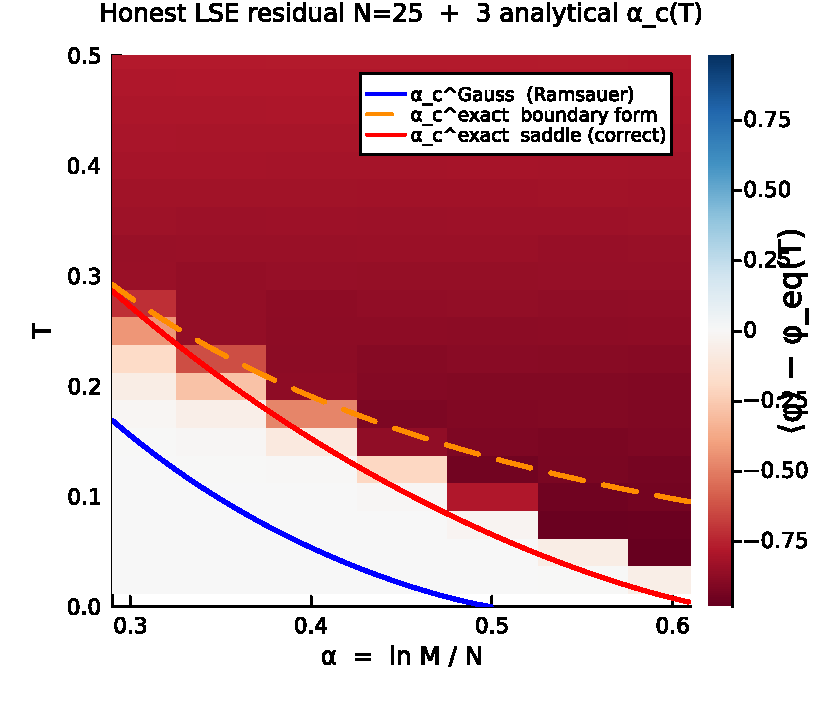
\includegraphics[width=0.92\linewidth]{panels_paper/heatmap_LSE_AAAI_residual_3boundaries.pdf}
\caption{Residual $\avg{\phi} - \phieq(T)$ of the honest and
semismart Monte Carlo at $N = 25$ over $\alpha\in[0.20,0.70]$,
$T\in[0.025,0.500]$, with the three analytical capacity boundaries from
\Cref{sec:formulas} overlaid: Gaussian (Ramsauer; blue solid), exact-density
boundary form (orange dashed), exact-density saddle form (red solid; this
work). Where both schemes converged at the same $(\alpha,T)$ cell the
residual is the mean of the two. The red curve tracks the white-to-red
transition zone for $\alpha\gtrsim0.45$; the blue Gaussian curve sits
deep inside the spin-glass region for the entire range; the orange
boundary form sits far outside, over-predicting capacity. The orange and
red curves meet near $(\alpha, T)\approx(0.241,\,0.36)$, in agreement
with the regime split \Cref{sec:formulas:split}.}
\label{fig:heatmap}
\end{figure}

\Cref{fig:heatmap} is the central empirical statement of the paper. Three
features deserve emphasis. First, the Gaussian boundary $\acGauss$
\eqref{eq:acgauss} sits far inside the spin-glass region for every
$\alpha$ in the range; the Ramsauer value $0.5$ is not the boundary one
sees in finite-temperature Monte Carlo at finite $N$. Second, the naive
transplant $\acBd$ \eqref{eq:acbd} sits far outside the empirical
transition, climbing to large $\alpha$ at modest $T$ and diverging at
$T\to 0$; it is the wrong boundary for LSE in essentially the entire
relevant $\alpha$ range, despite being the correct form for LSR. Third,
the saddle boundary $\acSd$ \eqref{eq:acsd} traces the white-to-red
transition zone for $\alpha \gtrsim 0.45$, the regime where the
candidate kinetic shift discussed in \Cref{sec:mc:smallalpha} is small.
At $\alpha < 0.45$ the empirical transition lies at lower $T$ than
$\acSd$ predicts. The crossover at $\alpha \approx 0.241$, $T\approx
0.36$ between the boundary form and the saddle form, predicted from
\Cref{sec:formulas:split}, is visible within the plotted range. Where
honest and semismart estimates coexist (the lower half of the $\alpha$
range) their residuals agree within Monte Carlo noise, indicating that
the semismart truncation faithfully reproduces the saddle-band physics
that drives the boundary.

% =========================================================================
\section{Conclusion}
\label{sec:conclusion}

Ramsauer et al.\ established the LSE capacity $\alpha_c = 0.5$ at zero
temperature, in a static argument that does not formalise basin stability
against thermal noise. The companion thermodynamic
analysis~\citep{icml2026theory} recovered the same value as the
$T\!\to\!0$ limit of a smooth phase boundary while retaining the Gaussian
approximation for the inter-pattern overlap distribution. The further
companion paper~\citep{petrova2026metastable} replaced the Gaussian by
the exact spherical density and showed that, for the compactly-supported
LSR kernel, the lighter tail of that density raises the threshold from
the Gaussian $\varphi_c^2/2$ to $-\tfrac12\ln(1-\varphi_c^2)$, a shift
from $0.25$ to $\approx 0.347$ at the canonical choice
$b = 2+\sqrt{2}$.

The natural question for LSE is settled by the observation that the
lighter-tail correction cannot be applied via the support boundary
alone. The exponential kernel of \eqref{eq:lse-energy} multiplies the
lighter-tail density by $\e^{\Bnet N \varphi}$, and the resulting
integrand develops an interior maximum at the golden ratio
$\varphi^{*} = (\sqrt{5}-1)/2$, with saddle value $g_{\max}\approx
0.3774$. The correct zero-temperature capacity for LSE is
$\Bnet - g_{\max}\approx 0.6226$, intermediate between Ramsauer's $0.5$
and the divergent boundary form one obtains by importing the LSR
formula without modification. The Ramsauer threshold of $0.5$ should be
reconsidered in this light: it is the Gaussian estimate of a quantity
that the exact spherical density assigns a strictly larger value.

LSR follows a qualitatively different rule. The ReLU kernel
$\max(0,\,1-b+b\,\varphi)$ has hard support $[\varphi_c,\,1]$. On this
interval the entropy density $(1-\varphi^2)^{(N-3)/2}$ is past its peak
(which sits at $\varphi=0$, outside the support) and monotonically
decreasing, and the kernel weight is linear rather than exponential. The
integrand of the LSR analogue of \eqref{eq:spurious-sum} is therefore
monotonically decreasing on $[\varphi_c, 1]$ and dominated by the
boundary at $\varphi_c$, with no interior saddle. The LSR threshold
$\approx 0.347$ is genuinely boundary-driven; the LSE threshold
$\approx 0.6226$ is genuinely saddle-driven. Kernel softness versus
hardness selects the regime.

Intermediate kernels (e.g.\ a smoothed ReLU with finite slope at
$\varphi_c$) interpolate between the two limits, and one may expect a
continuous family of capacity boundaries between the LSR
boundary-dominated and LSE saddle-dominated extremes. The
small-$\alpha$ discrepancy of \Cref{sec:mc:smallalpha} between the
empirical Monte Carlo transition and the saddle prediction admits at
least two candidate accounts: the LSE analogue of the LSR Kramers
shift of~\citep{petrova2026metastable}, and the single-pattern
spinodal of \Cref{sec:mc:spinodal}. The two predict opposite signs
for the residual $T_c^{\mathrm{app}} - T_c^{\mathrm{sd}}$ at large
$N$, so an $N$-scan past the present range together with a
two-initialisation test would identify which mechanism (if either)
dominates. Both interpretations remain conjectural until the
validation programme of \Cref{sec:mc:smallalpha} is executed.

\bibliographystyle{plain}
\bibliography{refs}

\end{document}
